% По умолчанию используется шрифт 14 размера. Если нужен 12-й шрифт, уберите опцию [14pt]
\documentclass[14pt, russian]{matmex-diploma-custom}
\usepackage[table]{xcolor}
\usepackage{graphicx}
\usepackage{tabularx}
\newcolumntype{Y}{>{\centering\arraybackslash}X}
\usepackage{amsmath}
\usepackage{amsthm}
\usepackage{amsfonts}
\usepackage{amssymb}
\usepackage{mathtools}
\usepackage{thmtools}
\usepackage{thm-restate}
\usepackage{tikz}
\usepackage{wrapfig}
% \usepackage[kpsewhich,newfloat]{minted}
% \usemintedstyle{vs}
\usepackage[inline]{enumitem}
\usepackage{subcaption}
\usepackage{caption}
\usepackage[nocompress]{cite}
\usepackage{makecell}
% \setitemize{noitemsep,topsep=0pt,parsep=0pt,partopsep=0pt}
% \setenumerate{noitemsep,topsep=0pt,parsep=0pt,partopsep=0pt}


\graphicspath{ {resources/} }

% 
% % \documentclass 
% %   [ a4paper        % (Predefined, but who knows...)
% %   , draft,         % Show bad things.
% %   , 12pt           % Font size.
% %   , pagesize,      % Writes the paper size at special areas in DVI or
% %                    % PDF file. Recommended for use.
% %   , parskip=half   % Paragraphs: noindent + gap.
% %   , numbers=enddot % Pointed numbers.
% %   , BCOR=5mm       % Binding size correction.
% %   , submission
% %   , copyright
% %   , creativecommons 
% %   ]{eptcs}
% % \providecommand{\event}{ML 2018}  % Name of the event you are submitting to
% % \usepackage{breakurl}             % Not needed if you use pdflatex only.
% 
% \usepackage{underscore}           % Only needed if you use pdflatex.
% 
% \usepackage{booktabs}
% \usepackage{amssymb}
% \usepackage{amsmath}
% \usepackage{mathrsfs}
% \usepackage{mathtools}
% \usepackage{multirow}
% \usepackage{indentfirst}
% \usepackage{verbatim}
% \usepackage{amsmath, amssymb}
% \usepackage{graphicx}
% \usepackage{xcolor}
% \usepackage{url}
% \usepackage{stmaryrd}
% \usepackage{xspace}
% \usepackage{comment}
% \usepackage{wrapfig}
% \usepackage[caption=false]{subfig}
% \usepackage{placeins}
% \usepackage{tabularx}
% \usepackage{ragged2e}
% \usepackage{soul}
\usepackage{csquotes}
% \usepackage{inconsolata}
% 
% \usepackage{polyglossia}   % Babel replacement for XeTeX
%   \setdefaultlanguage[spelling=modern]{russian}
%   \setotherlanguage{english}
% \usepackage{fontspec}    % Provides an automatic and unified interface 
%                          % for loading fonts.
% \usepackage{xunicode}    % Generate Unicode chars from accented glyphs.
% \usepackage{xltxtra}     % "Extras" for LaTeX users of XeTeX.
% \usepackage{xecyr}       % Help with Russian.
% 
% %% Fonts
% \defaultfontfeatures{Mapping=tex-text}
% \setmainfont{CMU Serif}
% \setsansfont{CMU Sans Serif}
% \setmonofont{CMU Typewriter Text}

\usepackage[final]{listings}

\lstdefinelanguage{ocaml}{
keywords={@type, function, fun, let, in, match, with, when, class, type,
nonrec, object, method, of, rec, repeat, until, while, not, do, done, as, val, inherit, and,
new, module, sig, deriving, datatype, struct, if, then, else, open, private, virtual, include, success, failure,
lazy, assert, true, false, end},
sensitive=true,
commentstyle=\small\itshape\ttfamily,
keywordstyle=\ttfamily\bfseries, %\underbar,
identifierstyle=\ttfamily,
basewidth={0.5em,0.5em},
columns=fixed,
fontadjust=true,
literate={->}{{$\to$}}3 {===}{{$\equiv$}}1 {=/=}{{$\not\equiv$}}1 {|>}{{$\triangleright$}}3 {\\/}{{$\vee$}}2 {/\\}{{$\wedge$}}2 {>=}{{$\ge$}}1 {<=}{{$\le$}} 1,
morecomment=[s]{(*}{*)}
}

\lstset{
mathescape=true,
%basicstyle=\small,
identifierstyle=\ttfamily,
keywordstyle=\bfseries,
commentstyle=\scriptsize\rmfamily,
basewidth={0.5em,0.5em},
fontadjust=true,
language=ocaml
}
 
\newcommand{\cd}[1]{\texttt{#1}}
\newcommand{\inbr}[1]{\left<#1\right>}


\newcolumntype{L}[1]{>{\raggedright\let\newline\\\arraybackslash\hspace{0pt}}m{#1}}
\newcolumntype{C}[1]{>{\centering\let\newline\\\arraybackslash\hspace{0pt}}m{#1}}
\newcolumntype{R}[1]{>{\raggedleft\let\newline\\\arraybackslash\hspace{0pt}}m{#1}}



\usepackage{soul}
\usepackage[normalem]{ulem}
%\sout{Hello World}

% перевод заголовков в листингах
\renewcommand\lstlistingname{Листинг}
\renewcommand\lstlistlistingname{Листинги}

\usepackage{afterpage}
\usepackage{pdflscape}
\usepackage{listings}
\usepackage{tikz}
\usetikzlibrary{decorations.pathreplacing,calc,shapes,positioning,tikzmark}

\newcounter{tmkcount}

\tikzset{
  use tikzmark/.style={
    remember picture,
    overlay,
    execute at end picture={
      \stepcounter{tmkcount}
    },
  },
  tikzmark suffix={-\thetmkcount}
}


\usepackage{caption}
\usepackage{listings}
\usepackage{hyperref}
\usepackage{xcolor}
\definecolor{linkcolor}{HTML}{001B12}
\definecolor{urlcolor}{HTML}{001B12}
\hypersetup{pdfstartview=FitH,  linkcolor=linkcolor,urlcolor=urlcolor, colorlinks=true}


\DeclareCaptionFont{white}{ \color{white} }
\DeclareCaptionFormat{listing}{
    \parbox{\textwidth}{\hspace{15pt}#1#2#3}
}
\captionsetup[lstlisting]{ format=listing
  %, labelfont=white, textfont=white
  , singlelinecheck=false, margin=0pt, font={bf}
}
\begin{document}
\large
%% Если что-то забыли, при компиляции будут ошибки Undefined control sequence \my@title@<что забыли>@ru
%% Если англоязычная титульная страница не нужна, то ее можно просто удалить.
\filltitle{ru}{
    %% Актуально только для курсовых/практик. ВКР защищаются не на кафедре а в ГЭК по направлению, 
    %%   и к моменту защиты вы будете уже не в группе.
    chair              = {Кафедра системного программирования},
    group              = {19.Б09-мм},
    %
    %% Макрос filltitle ненавидит пустые строки, поэтому обязателен хотя бы символ комментария на строке
    %% Актуально всем.
    title              = {Метрики кода для OCaml},
    % 
    %% Здесь указывается тип работы. Возможные значения:
    %%   coursework - отчёт по курсовой работе;
    %%   practice - отчёт по учебной практике;
    %%   prediploma - отчёт по преддипломной практике;
    %%   master - ВКР магистра;
    %%   bachelor - ВКР бакалавра.
    type               = {practice},
    %
    %% Здесь указывается вид работы. От вида работы зависят критерии оценивания.
    %%   solution - <<Решение>>. Обучающемуся поручили найти способ решения проблемы в области разработки программного обеспечения или теоретической информатики с учётом набора ограничений.
    %%   experiment - <<Эксперимент>>. Обучающемуся поручили изучить возможности, достоинства и недостатки новой технологии, платформы, языка и т. д. на примере какой-то задачи.
    %%   production - <<Производственное задание>>. Автору поручили реализовать потенциально полезное программное обеспечение.
    %%   comparison - <<Сравнение>>. Обучающемуся поручили сравнить несколько существующих продуктов и/или подходов.
    %%   theoretical - <<Теоретическое исследование>>. Автору поручили доказать какое-то утверждение, исследовать свойства алгоритма и т.п., при этом не требуя написания кода.
    kind               = {solution},
    %
    author             = {Белошапкин Михаил Юрьевич},
    % 
    %% Актуально только для ВКР. Указывается код и название направления подготовки. Типичные примеры:
    %%   02.03.03 <<Математическое обеспечение и администрирование информационных систем>>
    %%   02.04.03 <<Математическое обеспечение и администрирование информационных систем>>
    %%   09.03.04 <<Программная инженерия>>
    %%   09.04.04 <<Программная инженерия>>
    %% Те, что с 03 в середине --- бакалавриат, с 04 --- магистратура.
    specialty          = {02.03.03 <<Математическое обеспечение и администрирование информационных систем>>},
    % 
    %% Актуально только для ВКР. Указывается шифр и название образовательной программы. Типичные примеры:
    %%   СВ.5006.2017 <<Математическое обеспечение и администрирование информационных систем>>
    %%   СВ.5162.2020 <<Технологии программирования>>
    %%   СВ.5080.2017 <<Программная инженерия>>
    %%   ВМ.5665.2019 <<Математическое обеспечение и администрирование информационных систем>>
    %%   ВМ.5666.2019 <<Программная инженерия>>
    %% Шифр и название программы можно посмотреть в учебном плане, по которому вы учитесь. 
    %% СВ.* --- бакалавриат, ВМ.* --- магистратура. В конце --- год поступления (не обязательно ваш, если вы были в академе/вылетали).
    programme          = {СВ.5006.2017 <<Математическое обеспечение и администрирование информационных систем>>},
    % 
    %% Актуально только для ВКР, только для матобеса и только 2017-2018 годов поступления. Указывается профиль подготовки, на котором вы учитесь.
    %% Названия профилей можно найти в учебном плане в списке дисциплин по выбору. На каком именно вы, вам должны были сказать после второго курса (можно уточнить в студотделе).
    %% Вот возможные вариканты:
    %%   Математические основы информатики
    %%   Информационные системы и базы данных
    %%   Параллельное программирование
    %%   Системное программирование
    %%   Технология программирования
    %%   Администрирование информационных систем
    %%   Реинжиниринг программного обеспечения
    % profile            = {Системное программирование},
    % 
    %% Актуально всем.
    %supervisorPosition = {проф. каф. СП, д.ф.-м.н., проф.}, % Терехов А.Н.
    supervisorPosition = {к.т.н., доцент кафедры системного программирования}, % Григорьев С.В.
    supervisor         = {Ю.В. Литвинов},  
    consultantPosition = {программист <<JetBrains Labs>>},
    consultant         = {Д.С. Косарев},
    % 
    %% Актуально только для практик и курсовых. Если консультанта нет, закомментировать или удалить вовсе.
}
\maketitle
\newpage
\tableofcontents % Вывод содержания
\newpage
\section{Введение}
При разработке программных продуктов полезно иметь представление
о качестве исходного кода, а также об общей сложности проекта. 
Конечно, можно оценивать эти параметры и вручную, но в промышленной разработке такой подход недопустим, поэтому данный процесс необходимо автоматизировать с помощью метрик кода.

Метрика кода -- это некоторая численная мера, которая оценивает определенные свойства конкретного участка программного кода. При этом для каждой конкретной метрики существует эталон, при сильном отклонении от которого рекомендуется произвести рефакторинг. Метрики оценивают разные аспекты программы: сложность и структурированность, связность компонентов, объем компонентов. Эти и многие другие показатели позволяют предварительно оценить корректность реализации той или иной части проекта.

Для объектно-ориентированных и процедурных языков метрики реализованы в большинстве сред разработки, однако для некоторых функциональных языков на данный момент просто не существует инструментов, которые позволяли бы определять качество кода на основе ряда показателей. В качестве примера можно привести OCaml -- наиболее популярный язык семейства ML. Как новичкам, так и опытным разработчикам было бы не лишним знать, насколько сложным
является их проект и насколько качественно он реализован,  поэтому было принято решение разработать инструмент, расчитывающий метрики кода для OCaml.

\section{Постановка задачи}
Целью работы является разработка прототипа инструмента, позволяющего вычислять метрики кода для OCaml. Для достижения данной цели были сформулированы следующие промежуточные задачи:
\begin{enumerate}
    \item Сделать обзор различных метрик.
    \item Сделать обзор существующих аналогов.
    \item Разработать прототип инструмента для подсчета метрик.
    \item Провести тестирование инструмента.
\end{enumerate}
\section{Обзор}
Для реализации были выбраны SLOC, метрика
Холстеда, а также цикломатическая сложность, так как при 
создании инструментов анализа кода они используются наиболее часто.
\subsection{SLOC}
Количественные метрики базируются на оценке объема различных компонентов программы. Наиболее распространненным примером является SLOC-метрика\footnote{Вся информация о
SLOC-метриках взята из статьи Lines Of Code Metrics. https://www.aivosto.com/project/help/pm-loc.html (Date: 07.03.2022)} (Source Lines Of Code). Самый тривиальный пример SLOC-оценки -- это количество физических строк в проекте. Однако этот показатель сам по себе мало информативен, к тому же в зависимости от стиля программирования может меняться количество строк, реализующих одну и ту же функциональность, поэтому вместе с физическими строками полезно считать и логические строки (LLOC -Logical lines of code),то есть строки, которые содержат что-то помимо пробелов, скобок, символов разделителей и комментариев. В то же время неплохо иметь представление о качестве документирования, поэтому были введены оценки LLOC' (Logical Lines of Comments)
и MCOMM (Meaningful Comments). Значение LLOC' равно общему количеству строк с комментариями, MCOMM -- количеству строк с комментариями, которые имеют текстовое содержание. При этом на пять строк к комментариями должна приходиться минимум одна
строка с текстовым содержанием. 

Вышеперечисленные значения можно варьировать и вычислять другие метрики. Также полезно оценивать размер отдельных процедур и классов (например, наличие функции в 500 строк может говорить о проблеме с декомпозицией). Граничные
показатели SLOC-метрик могут меняться в зависимости от языка, ниже в таблице  представлены рекомендуемые размеры компонентов для Java: 
\begin{center}
\begin{tabular}{ | c | c | c | c | }
\hline
    & Procedure LLOC &  Class LLOC & File LLOC \\ \hline 
min & 3         & 3      & 1 \\  \hline
max & 50        & 1500   & 2000\\ \hline
\end{tabular}
\end{center}

Для OCaml и других функциональных языков на данный момент не существует 
эталонных значений для вышеописанных оценок, однако учитывая то, что для данного типа языков используется декларативный стиль программирования, рекомендуемый максимум для метрик должен быть меньше.
\subsection{Метрика Холстеда}
Метрика Холстеда позволяет оценить сложность определённого участка кода на основе 
четырех показателей: общее количество операторов $N_1$ (в множество операторов также входят символы-разделители и ключевые слова), общее количество операндов $N_2$, количество уникальных операторов $n_1$, количество уникальных операндов $n_2$. Сюда же добавляют теоретическое число уникальных операторов $n_1'$ и теоретическое число уникальных операндов $n_2'$. С помощью вышеописанных данных вычисляют следующие значения\footnote{Милютин А. Статья <<Метрики кода программного обеспечения>>}:
\begin{center}
\begin{tabular}{|l l|}
\hline
$n = n_1 + n_2$ &-- словарь программы.
\\
$n' = n_1' + n_2'$ &-- теоретический словарь программы.
\\
$N = N_1 + N_2$ &-- длина программы.
\\
$N' = n_1 \log_{2} n_1 + n_2 \log_{2} n_2$ &-- теоретическая длина программы.
\\
$V = N\log_2 n$ &-- объём программы.
\\
$V'= N\ \log_2 n'$ &-- теоретический объём программы.
\\
$L = \frac{V'}{V}$ &-- уровень качества программирования.
\\
$L' =\frac{2}{n_1} \cdot \frac{n_2}{N_2}$ &-- уровень качества программирования 
\\ & (без учёта теоретических параметров). 
\\
$D = \frac{1}{L'}$ &-- трудоёмкость кодирования.
\\
$I = \frac{V}{D}$ &-- информационное содержание программы.
\\\hline
\end{tabular}
\end{center}
Анализируя получившиеся результаты, можно определить трудоемкость разработки, сложность понимания программы, информационное содержание программы. При этом
для стилистически корректного кода отклонение длины от теоретической длины не должно превышать 10 \%, а для идеальной программы значение уровня качества программирования равно единице.  
\subsection{Цикломатическая сложность}
Цикломатическая сложность (или метрика Мак-Кейба) -- наиболее известная
метрика для оценки сложности программ. Она показывает число линейно независимых маршрутов
через программный код, то есть если, к примеру, участок кода не содержит операторов ветвления, цикломатическая сложность равна единице, если содержит одну условную конструкцию
if-else -- цикломатическая сложность равна двум. Данная метрика 
вычисляется с помощью графа потока управления (Control Flow Graph) 
определенного участка кода (чаще всего это модули, классы или методы, однако цикломатическая сложность может быть расчитана и для всего проекта в случае, если построен общий граф потока управления на основе графа вызовов).
Графом	потока управления программы называется ориентированный граф,	 в	узлах	которого находятся	неделимые группы	команд,	а ребрами	соединяются такие	блоки,	которые	могут	быть	выполнены	
сразу	друг	за	другом. Цикломатическая сложность графа, который имеет
$e$ дуг, $n$ вершин и $p$ компонент связности, 
расчитывается по формуле\footnote{T.J. McCabe, <<A Complexity Measure>>}: $V = e - n + 2p$.  

Данный показатель позволяет оценить различные параметры: насколько трудоёмкой является реализация той или иной части проекта, насколько сложно осуществлять поддержку и изменение кода, какое количество тестов необходимо для полного покрытия.

В качестве недостатков можно отметить то, что метрика Мак-Кейба не различает
циклы и условные конструкции, не учитывает наличие рекурсивных функций,
а также игнорирует сложность предикатов. Но несмотря на это цикломатическая сложность широко используется как в качестве самостоятельной метрики, так и в составе гибридных метрик, что обуславливается простотой её реализации.

До сих пор не принята единая рекомендуемая верхняя граница цикломатической сложности. Так, авторы Microsoft Docs\footnote{https://docs.microsoft.com/ru-ru/dotnet/fundamentals/code-analysis/quality-rules/ (Date: 20.03.2022)}  принимают это число равным 25, а разработчики Project Analyzer
рекомендуют писать фунции с ц. сложностью, не превышающей десяти.
\subsection{Cognitive Complexity}
На практике можно довольно часто встретить ситуацию, когда цикломатическая сложность
не является эффективной метрикой. Рассмотрим следующий пример:
\\
\\
\\
Значения цикломатической сложности обеих функций равны, однако очевидно, что код слева интуитивно менее понятен, чем код справа. Поэтому появилась необходимость в сзоздании новой метрики, которая бы позволяла производить оценку сложности.
Значение Cognitive Complexity вычисляется по изложенным ниже правилам.
\begin{itemize}
    \item Каждое прерывание потока управления увеличивает значение Cognitive Complexity на единицу
    \item Вложенные конструкции (например, if внутри цикла) увеличивают значение Cognitive Complexity на единицу 
\end{itemize}
Учитывается рекурсия
\newpage
\subsection{Существующие решения}
\textbf{Rust-code-analysis.} Статический анализатор кода с открытым исходным кодом, написанный на Rust. Вычисляет метрики для Python, JavaScript, TypeScript, Rust, C++. Реализует оценку 
цикломатической сложности, SLOC, метрики Холстеда, а также расчитывает значение Cognitive-Complexity\footnote{В некоторых случаях оценка с помощью цикломатическая сложности не является корректной. Для решения данной проблемы компанией Sonar была разработана новая метрика Cognitive Complexity 
\\https://redirect.sonarsource.com/doc/cognitive-complexity.html (Date: 19.03.2022)}. Вычисления проводятся посредством анализа абстрактного синтаксического дерева, построение которого
реализуется внутри проекта. При этом вычисление цикломатической сложности
производится по упрощенному алгоритму -- без построения CFG, -- путем подсчета
общего количества условных операторов.

\textbf{Radon.} Консольная утилита, позволяющая вычислять метрики для Python. Расчитывает SLOC, цикломатическую сложность, метрику Холстеда, а также Maintainability Index\footnote{Значение Maintainability Index расчитывается на основе цикломатической сложности, SLOC и объема программы по Холстеду. https://radon.readthedocs.io/en/latest/intro.html\#maintainability-index (Date: 25.03.2022)} -- программную метрику, которая показывает, насколько 
легким в поддержке является исходный код. По аналогии с Rust-code-analysis 
цикломатическая сложность считается без построения CFG.

\textbf{Visual Studio}. Visual Studio содержит
встроенные инструменты для анализа кода .NET
платформы, в том числе и метрики, среди которых\footnote{https://docs.microsoft.com/ru-ru/visualstudio/code-quality/code-metrics-values?view=vs-2022 (Date: 03.04.2022)}:
SLOC, Maintainability Index, цикломатическая сложность, глубина наследования, метрики взаимосвязи
классов.

\textbf{Project Analyzer} -- анализатор кода для Visual Basic. Помимо инструментов, позволяющих обнаружить слабые места в проекте (неиспользуемый, неоптимизированныый, дублирующий  код, стилистические и логические ошибки), реализует 184 метрики, такие как SLOC, цикломатическая сложность, глубина наследования, качество документирования, стилистические метрики (например, проверяющие корректность имен переменных), а также объектно-ориентированные метрики.
\section{Реализация}
В качестве основы проекта был взят линтер\footnote{https://github.com/Kakadu/zanuda}, в котором
уже были реализованы некоторые модули. Для расчета метрик кода для OCaml были использованы
библиотеки compilier-libs\footnote{compilier-libs-- библиотека, реализующая инструменты для построения и анализа AST, Typed AST,  является частью внутреннего API компилятора OCaml,\\
https://ocaml.org/api/compilerlibref/Compiler\_libs.html (Date: 02.04.2022)} (для построения и анализа AST) и Lexing\footnote{Lexing -- библиотека для работы с лексерами и парсерами\\ https://ocaml.org/api/Lexing.html (Date: 02.04.2022)} (для анализа текста программ), так как они хорошо документированы и содержат все
необходимые инструменты. Вся информация о собранных метриках записывается в модуль StatisticsCollector. SLOC-метрики вычисляются в модуле LOC, метрика Холстеда 
-- в модуле Halstead, цикломатическая сложность -- в модуле CCComplexity, построение
графа потока управления осуществляется в модуле CFG.
\begin{figure}[h]
    \center{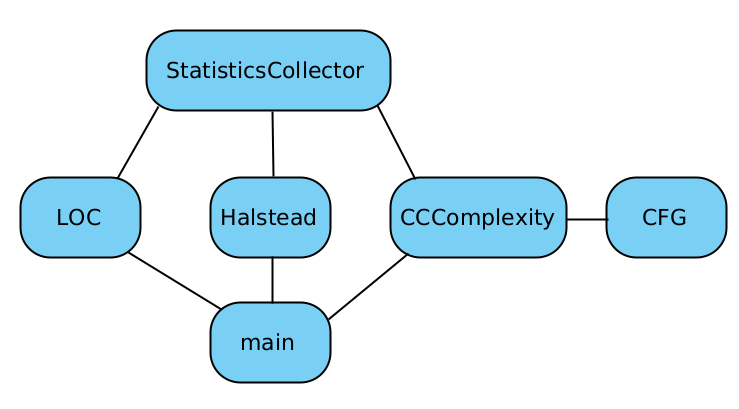
\includegraphics[scale=0.5]{data.png}}
    \caption{Модульная структура программы}
\end{figure}

\subsection{Метрики}
При вычислении базовых LOC-метрик мы можем работать непосредственно с текстом программы,
так как на данном этапе нам не обязательно иметь представление о семантике OCaml. Для анализа кода создаём лексер, реализующий три правила разбора: для логических строк (logic), комментариев (comments) и <<пустых>> строк (empty), а также считающий их количество. Пустая строка -- это строка, которая содержит только пробелы, табуляцию, символы разделители и скобки, в нашем случае она задается регулярным выражением.
Значения SLOC вычисляются в модуле LOC, откуда передаются в StatisticsCollector.

Для расчета метрики Холстеда уже появляется необходимость
анализировать структуру кода. Для этого с помощью модуля \\ Compile\_common\footnote{Compile\_common -- модуль библиотеки compilier-libs\\  https://docs.mirage.io/ocaml/Compile\_common/index.html (Date:12.03.2022)} строится типизированное абстрактное синтаксическое дерево (Typed AST). Нам интересно вычислять данную метрику отдельно для каждой функции в модуле: во-первых, оценка всего модуля будет не информативна, так как не покажет слабых мест в коде, во-вторых, так появляется возможность сравнить две реализации
одной и той же функции. Для реализации данной идеи с помощью модуля Tast\_iterator\footnote{Tast\_iterator -- модуль библиотеки
Compilier-libs, позволяющий реализовать итератор для обхода типизированного абстрактного синтаксического дерева.\\https://docs.mirage.io/ocaml/Tast\_iterator/index.html (Date: 12.03.2022)} в функции run создаем
итератор, который работает следующим образом: если текущая вершина -- это выражение, описывающее функцию, создаётся 
новый итератор, который совершает обход синтаксического дерева данной функции и
собирает данные об операторах и операндах. После завершения обхода полученные
результаты передаются в StatisticsCollector.

Для вычисления метрики Мак-Кейба существует два подхода: первый -- через граф потока управления, второй -- через подсчёт количества условных операторов (то есть цикломатическая сложность равна числу условных операторов плюс один, так, например, реализовано в Rust-code-analyzis и Radon). Очевидно, что второй подход
проще, поэтому было принято решение сначала реализовать его.  
Используется тот же алгоритм, что и для метрики Холстеда, только в данном случае
считаются только условные операторы (if-then-else, match, function, for, while,
try-with). Для реализации первого подхода необходимо получить граф потока управления функции из выражения Parsetree.expression, но библиотека compilier-libs на данный момент такую возможность не предоставляет, поэтому было принято решение
реализовать отдельный модуль, в котором и будет строиться CFG.

\subsection{Control Flow Graph}
Для вычисления цикломатической сложности нам необходимо
по выражению, описывающему функцию, построить граф потока
управления этой функции. Данная процедура реализуется в функции build\_cfg модуля CFG. В нашем случае необязательно строить точный граф, где каждый узел является неделимым набором инструкций, интерес представляет только его
топологическая структура. Поэтому мы можем строить
упрощенную модель CFG\footnote{https://microeducate.tech/get-control-flow-graph-from-abstract-syntax-tree/ (Date: 15.03.2022)}: если выражение не содержит ветвлений, то в графе для
него создается один узел. Если текущая вершина AST -- это условый оператор, то производится обход дочерних узлов, после которого в графе создается вершина,
замыкающая ветвление. Данный процесс повторяется до полного прохода AST.
\section{Тестирование}
Для проверки корректности реализованных метрик было применено ручное тестирование
с использованием как простых примеров кода, так и исходников проекта.  Для каждой
метрики была создана директория с тестируемым кодом и файлом run.t, который содержит
скрипт, запускающий тесты. Метрика Мак-Кейба проверялась на случайных функциях из проекта, на функциях без ветвлений, а также на функциях, содержащих несколько вложенных
условных конструкций (например, function, внутри которого if, внутри которого match). 
Корректность LOC-оценок проверялась на исходном коде проекта. Тестирование метрики Холстеда
показало необходимость доработки, так в ряде случаев полученный набор операторов и операндов
не является полным (например, при разборе оператора match не анализируется левая часть выражений, описывающая паттерны).

Помимо случайных примеров кода из проекта нам бы также хотелось проанализировать какую-нибудь
содержательную программу: во первых, для того, чтобы протестировать инструмент, и во-вторых, чтобы
сравнить OCaml с императивными языками, реализующими тот же алгоритм. В качестве такого
примера было реализовано обычное дерево бинарного поиска, АВЛ дерево, B-дерево. Результаты метрик 
представлены в таблицах:

\newpage
\section{Заключение}
Были получены следующие результаты:
\begin{enumerate}
    \item Сделан обзор различных метрик.
    \item Сделан обзор существующих аналогов.
    \item Разработан прототип\footnote{https://github.com/MihailBeloshapkin/mylinter} инструмента для подсчета метрик.
    \item Проведено тестирование инструмента.
\end{enumerate}

\newpage 
\begin{thebibliography}{9}
\bibitem{Metrics}
Милютин А. (2009) \emph{<<Метрики кода программного обеспечения>>} //-- (Date: 15.02.2022)
\bibitem{CC} 
T.J. McCabe, \emph{<<A complexity measure>>}, IEEE Transactions on
Software Engineering, vol. SE-2, no. 4, pp. 308-320, December,
1976 //- (Date: 25.02.2022)
\bibitem{OCaml} OCaml documentation: \emph{compilier-libs} //-- (Date: 26.02.2022) https://docs.mirage.io/ocaml/index.html
\bibitem{OCamllex} OCaml documentation: \emph{Lexing} //-- (Date: 20.03.2022)
https://ocaml.org/api/Lexing.html
\bibitem{Collisiom} Project analyzer documentation: \emph{Lines Of Code Metrics} //-- (Date: 23.02.2022) https://www.aivosto.com/project/help/pm-loc.html
\bibitem{SPA} Static Program Analysis //-- (Date: 26.03.2022)
http://www.cs.kent.edu/~jmaletic/cs63901/lectures/StaticAnalysis.pdf
\bibitem{CFG} Get Control Flow Graph from Abstract Syntax Tree //-- (Date: 28.03.2022)
https://microeducate.tech/get-control-flow-graph-from-abstract-syntax-tree/
\bibitem{Cogn} Cogitive Complexity. A new way of measuring understandability 
//- (Date: 14.08.2022) https://www.sonarsource.com/docs/CognitiveComplexity.pdf
\end{thebibliography}
\end{document}